%!TEX root = etdrtemplate.tex

\cleardoublepage


\chapter{PCA Pump}
\label{pcapump}

% http://www.santoslab.org/pub/paper/LarsonEtAl13-PCA-Requirements-SEHC-preprint.pdf
% http://ppahs.org/2012/05/30/patient-controlled-analgesia-pca-pumps-the-basics/

\begin{wrapfigure}{r}{0.4\textwidth}
  \begin{center}
    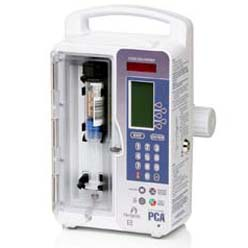
\includegraphics[width=0.4\textwidth]{figures/pca-pump.png}
  \end{center}
  \caption{Patient Controlled Analgesia (PCA) pump}
  \label{figure:pca-pump}
\end{wrapfigure}

Patient Controlled Analgesia (PCA) pump is a medical device, which allows the patient to self-administer small doses of narcotics (usually Morphine, Dilaudid, Demerol, or Fentanyl). PCA pumps are commonly used after surgery to provide a more effective method of pain control than periodic injections of narcotics. A continuous infusion (called a basal rate) permits the patient to receive a continuous infusion of pain medication. Patient can also request additional boluses, but only in specified intervals. It prevents from overinfusion. In addition to basal and patient bolus, clinician can also request bolus called clinician bolus or square bolus. 

Figure \ref{figure:pca-pump} shows LifeCare PCA pump. On the left hand side, there is drug reservoir. On the right, there is clinician panel, which allows to control the pump. Figure \ref{figure:alaris-pump} shows PCA Pump, made by company Alaris. 

\begin{wrapfigure}{l}{0.4\textwidth}
  \begin{center}
    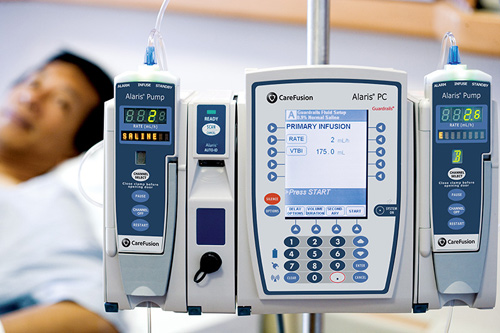
\includegraphics[width=0.4\textwidth]{figures/alaris-pump.png}
  \end{center}
  \caption{Alaris Pump}
  \label{figure:alaris-pump}
\end{wrapfigure}

PCA Pump is safety-critical device which works in standard process control loop depited in the figure \ref{figure:control-loop}. The controller obtains information about (observes) the process state from measured variables (feedback) and uses this information to initiate action by manipulating controlled variables to keep the process operating within predefined limits or set points (the goal) despite disturbances to the process. In general, the maintenance of any open-system hierarchy (either biological or man-made) will require a set of processes in which there is communication of information for regulation or control. \cite{SaferWorld} 

\begin{figure}[ht]%t=top, b=bottom, h=here
    \begin{center}
    	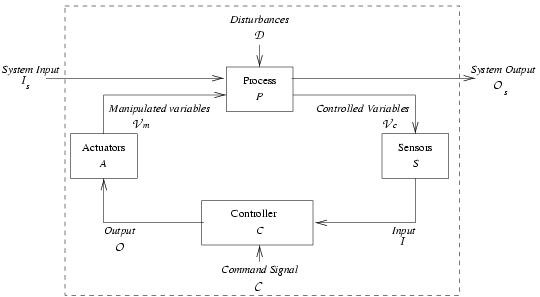
\includegraphics[width=0.9\textwidth]{figures/safety-critical-loop.png}    	
    \end{center}
    \caption{Standard Process Control Loop.}
    \label{figure:control-loop}
\end{figure}

PCA Pump actuator is motor, which pump drug to the patient's vein. Controlled process is dosing the drug. Sensors measure amount of dosed drug. They might be used for double-check if ordered (by controller) amount of drug was appropriately delivered. Sometimes there might be some distrubances caused by mechanical issues and environmental conditions. Controller issues appropriate actions based on informations from sensors and clinician or patient's commands. High level overview of PCA Pump is depicted in figure \ref{figure:pca-pump-system}.

\begin{figure}[ht]%t=top, b=bottom, h=here
    \begin{center}
    	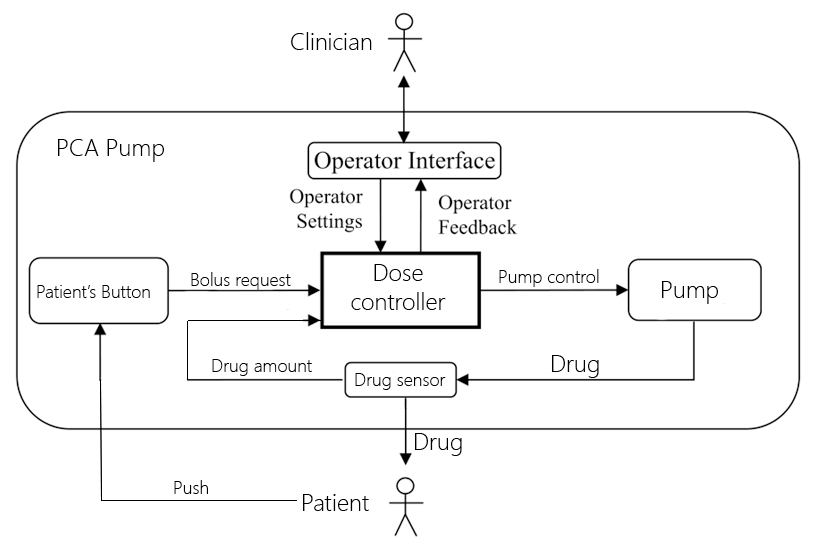
\includegraphics[width=0.9\textwidth]{figures/pca-pump-system.png}    	
    \end{center}
    \caption{PCA Pump system}
    \label{figure:pca-pump-system}
\end{figure}

One of the hazards of using PCA pumps, is that there is inadequate monitoring of patient's levels of oxygen and carbon dioxide. Nursing staff on general medical units typically track respiration rate and other vital signs every four hours, which is not enough. There should be a way to monitor levels continuously. Additionally, it can be hard to tell if a person's breathing rate is dangerously low in certain circumstances. There are cases, where lack of monitoring carbon dioxide level cause death.\footnote{http://abcnews.go.com/Health/parents-warn-pca-pumps-daughters-death/story?id=16796805} 

Another hazard is human mistake. For example, there is a case when nurse used a 5 mg/mL morphine cassette because a 1 mg/mL cassette was not available, but she programmed PCA Pump like for 1 mg/mL concentration. In addition to lack of monitoring of the pulse, patient died.\footnote{http://webmm.ahrq.gov/case.aspx?caseID=291}

As mentioned in chapter \ref{background}, the solution to that problem is medical devices interoperability. 

% use 890 .doc


\section{PCA Pump Requirements Document}
\label{pcapump:requirements-doc}

Requirements document \cite{PcaReq}.
Requirements document overview \cite{OpenSourcePCAPump:Paper}.

There can be situations in which the maximum drug amount induced may exceed the limit. E.g. when clinician issues too long square bolus. In such case, the Pump is switched to Keep Vein Open (KVO) mode, which has 1ml/hr drug rate. From this state pump has to be restarted by clinician. In Summary, Open PCA Pump has following modes:
\begin{itemize}
    \item Stopped
    \item Basal rate
    \item Bolus
    \item Clinician bolus (Square bolus)
    \item Keep Vein Open (KVO)
\end{itemize}

All information needed for Pump to operate should be specified by physician in the prescription, which is entered into PCA Pump. The prescription contains:
\begin{itemize}
    \item basal rate
    \item volume to be infused during patient bolus
    \item minimum time between patient boluses
    \item maximum drug amount allowed per hour
\end{itemize}

% state machine image?
% check UMinn document




\section{PCA Pump AADL/BLESS Models}
\label{pcapump:aadl-bless-models}
Selected modules for implementation. Pictures etc.



\section{BeagleBoard-XM}
\label{pcapump:beagleboard}
First step was create PCA Pump prototype on BeagleBoard-xM.

BeagleBoard-xM is Embedded device with AM37x 1GHz ARM processor (Cortex-A8 compatible). It has 512 MB RAM, 4 USB 2.0 ports, HDMI port, 28 General-purpose input/output (GPIO) ports and Linux Operating System (on microSD card). Moreover there is PWM support. All these properties makes this device good candidate for prototyping PCA Pump.

Pulse width modulation (PWM) is a technique for controlling analog circuits with a processor's digital outputs.

Expansion port 14(PWM) and 28(GND?)
GPIO158
Java Program to Run the pump for 10 seconds

There is no existing SPARK Ada compiler running on ARM system. Hence, to compile SPARK Ada program for ARM device, we need to perform cross-compilation on other machine. There is GNAT compiler \cite{Horn:Thesis} created by AdaCore, but there was no cross-compiler for ARM. However AdaCore was working on it. They had working version in 2013, but tested only on their target, Android-based device. BeagleBoard-xM is coming with Linux Angstrom Operating System. There is possibility to install Android on BeagleBoard-xM, but still not warranty everything will be working. Cooperation with AdaCore allowed to cross-compile SPARK Ada program for BeagleBoard-xM.

Include source of simple program?
GNAT cross-compiler only for Linux Platform (cross-compilation has to be done on Linux).

compilation+linking command: \lstinline{arm-linux-gnueabi-gnatmake -d -Ppca_ravenscar.gpr}.

%describe how to run the program: compile cmd with arm-gnuaebi... then copy to the board etc.



\section{Interface for Integrated Clinical Environment}
\label{pcapump:implementation:ice}

PCA Pump will be connected to ICE. It will allow to monitor and control device by MDCF (ICE implementation).
Describe communication with MDCF/ICE. PCA Pump ports for that etc.